\documentclass{article}
\usepackage[%
    left=0.5in,%
    right=0.5in,%
    top=0.5in,%
    bottom=0.5in,%
]{geometry}%
\usepackage{minitoc}
\usepackage{multicol}
\usepackage{graphicx}
\usepackage{fixltx2e}
\usepackage{hyperref}
\usepackage{hyperref}
    \hypersetup{ colorlinks = true, linkcolor = blue }
\usepackage{blindtext}

\graphicspath{ {./} }

\newcommand{\inlinecode}[2]{\colorbox{lightgray}{\lstinline
[language=#1]$#2$}}
\newcommand{\worddef}[1]{\hyperref[sec:reference]{\textit{#1}}}

\begin{document}

\section{Log structured file system}
\begin{flushleft}
Consider the \textbf{creation} of a new file on a Unix system:
\begin{itemize}
	\item \textbf{Allocate, initialise and write} the i-node for the file i-nodes are usually located at the start of the disk
	\item \textbf{Update} and write the directory entry for the file (directories are tables/files that map names onto i-nodes in Unix)
	\item Write the data to the disk 
\end{itemize}
The corresponding blocks \textbf{are not} necessarily in adjacent locations! Also in linked lists/FAT file systems blocks can be distributed \textbf{all over} the disk.
\end{flushleft}
\bigskip
\begin{flushleft}
Due to seek and \textbf{rotational delays}, hard disks are \textbf{slow} compared to other components in a computer (e.g. CPU, main memory).\textbf{Can we develop a file system that copes better with the inherent delays of traditional disks?}.\\
A \textit{log structured file system} aims to improve speed of a file system on a traditional hard disk by \textbf{minimising} head movements and rotational delays using \textbf{the entire disk} as a great big log. A log is a data structure that is written \textbf{only} at the end
\end{flushleft}

\subsection{Context}
\begin{flushleft}
\textit{Log structured} file systems \textbf{buffer read and write operations} (i-nodes, data, etc.) in memory, enabling us to write \textbf{“larger volumes}” in one go. Once the buffer is full it is “\textbf{flushed}” to the disk and written as one contiguous segment at the end of “a log”. I-nodes and data are all written to the \textbf{same segment} .Finding i-nodes (traditionally located at the start of the partition) becomes more difficult An \textbf{i-node map} is maintained in memory to quickly find the address of i-nodes on the disk
\end{flushleft}
\begin{center}
	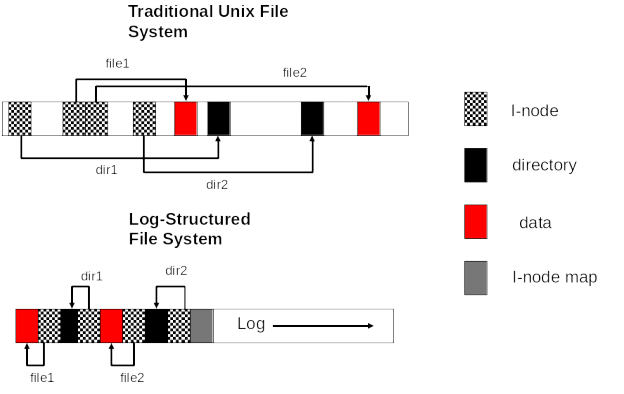
\includegraphics[scale=0.5]{log_fs.png}
\end{center}

\subsection{Deleting files}
\begin{flushleft}
\textbf{A cleaner thread} is running in the background and spends its time \textbf{scanning} the log circularly and \textbf{compacting} it. A hard drive is treated as a \textbf{circular buffer}. It \textbf{removes} deleted files and files being used right now are marked as \textbf{free segments} as they will be later written at the end.
\end{flushleft}

\subsection{Advantages and dissadvantages}
\begin{flushleft}
It greatly \textbf{increases} disk performance on writes, file creates, deletes. Writes are more \textbf{robust} as they are done as a \textbf{single operation}. (Multiple small writes are more likely to expose the file system to serious inconsistency). However, it has not been widely used because it is \textbf{highly incompatible} with existing file systems. In addition, the cleaner thread takes \textbf{additional} CPU time
\end{flushleft}

\section{Journaling file systems}
\begin{flushleft}
\textit{Journaling file systems} aim at increasing the \textbf{resilience} of file systems against crashes by \textbf{recording} each update to the file system as a \textbf{transaction}.
\end{flushleft}

\subsection{Concept}
\begin{flushleft}
The key idea behind a \textit{journaling file system} is to \textbf{log all events} (transactions) \textbf{before} they take place.
\begin{itemize}
	\item Write the actions that should be undertaken to a log file
	\item Carry them out
	\item Remove/commit the entries once completed 
\end{itemize}
If a crash happens in the \textbf{middle} of an action (e.g., deleting a file) the entry in the log file \textbf{will remain} present after the crash. The log can be examined after the crash and used to \textbf{restore} the consistency of the file system. \textbf{NTFS} and \textbf{EXT3-4} are examples of journaling file systems.
\end{flushleft}

\section{Virtual file systems}
\begin{flushleft}
Multiple file systems usually \textbf{coexist} on the same computer. These file systems can be seamlessly integrated by the operating system (e.g. Unix / Linux). This is usually achieved by using \textbf{virtual file systems} (VFS). VFS relies on standard object oriented principles (or manual implementations thereof), e.g. \textbf{polymorphism}. We devine a \textbf{generalised} interface that abstracts different file type implementations.\bigskip

In a similar way, Unix and Linux \textbf{unify} different file systems and present them as a \textbf{single hierarchy} and hides away / abstracts the implementation specific details for the user. The VFS presents a \textbf{unified interface} to the “outside”. File system specific code is dealt with in an \textbf{implementation layer} that is clearly separated from the interface.\bigskip

The VFS interface commonly contains the \textbf{POSIX} system calls (open, close, read, write, . . . ). Each file system that meets the VFS requirements provides an \textbf{implementation} for the system calls contained in the interface. Note that implementations can be for \textbf{remote file systems} (e.g. sshfs), i.e. the file can be stored on a different machine
\end{flushleft}

\subsection{Real word applications}
\begin{flushleft}
Every file system, including the \textbf{root file system}, is \textbf{registered} with the VFS.
\begin{itemize}
	\item A list / table of addresses to the VFS function calls (i.e. function pointers) for the specific file system is provided
	\item Every VFS function call corresponds to a specific entry in the VFS function table for the given file system
	\item The VFS maps / translates the POSIX call onto the “native file system call” 
\end{itemize}
A virtual file system is essentially \textbf{good programming practice}
\end{flushleft}

\pagebreak
\section*{Reference section} \label{sec:reference}
\begin{description}
	\item[placeholder] \hfill \\
\end{description}
\end{document}
